\section{Risultati}
\label{sec:risultati}
In questa sezione si valuteranno le performance dell'algoritmo.
Per condurre questa analisi si è generata una mappa di dimensioni note, come  in
figura \ref{fig:maptest}, si sono eseguiti dei test in diverse configurazioni
di tempo (da 200 \si{\second} a 1800 \si{\second}) e numero di robot
(da 1 a 4).
\begin{figure}[!htb]
	\centering
	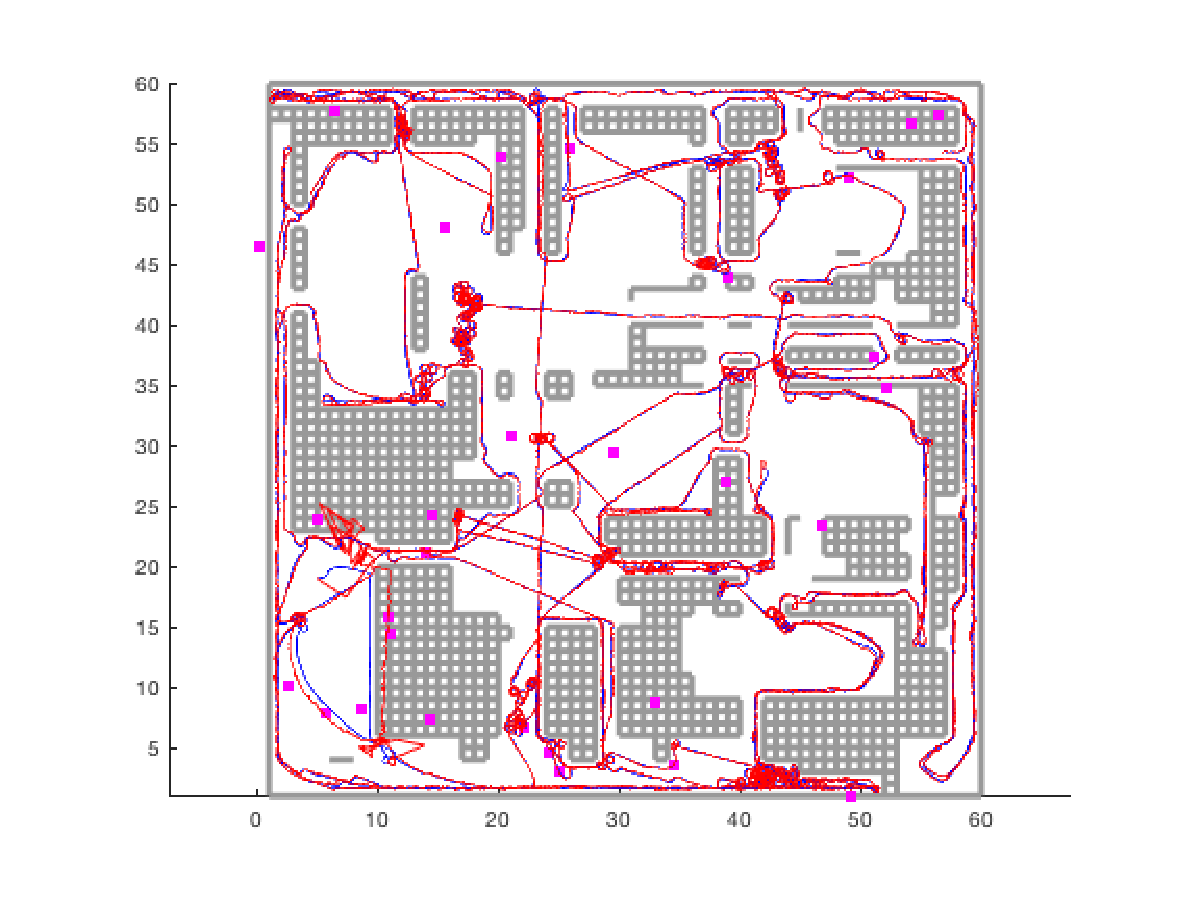
\includegraphics[width=\linewidth]{ParticleFilter}
	\caption{risulato simulazione mappa $60\times60$}
	\label{fig:maptest}
\end{figure}
All'interno della mappa di figura \ref{fig:maptest} sono riportate in blu le
traiettorie compiute dai robot nel caso ideale mentre in rosso le traiettorie stimate.
Le traiettorie riportate sono quelle ottenute da una simulazione di 1800
secondi e tramite l'utilizzo di tre robot che contemporaneamente la esplorano.
La scelta di tale numero di robot e tempo di simulazione è stata compiuta per
rispondere a due quesiti principali: efficienza energetica e percentuale di
mappa esplorata.
In figura \ref{fig:TotalDistance} si può condurre il primo tipo di studio
considerando che il percorrere una distanza maggiore comporta un maggiore
dispendio energetico mentre in figura \ref{fig:ExploredMap} si può notare come
spesso l'adottare un numero maggiore di robot porti ad un'esplorazione più
veloce.
Osservando entrambi i grafici si può evidenziare che l'adozione di quattro robot
rispetto a tre non comporti grossi benefici in termini di esplorazione
percentuale della mappa, ricade allora sul numero di 3 robot la nostra scelta in
quanto come evidenziato dal grafico \ref{fig:TotalDistance} questo comporta un
dispendio energetico minore.
Mentre il tempo totale di 1800 secondi è stato scelto in quanto a tale lunghezza
della  simulazione si ottiene un valore ragionevole di mappa esplorata $70\%$.
La percentuale di mappa esplorata è stata ottenuta considerando il numero totale
di celle libere realmente a disposizione rispetto al numero di celle viste dal
robot, come riportato nella equazione \eqref{eq:FracMap}.
%
\begin{equation}
Mappa Esplorata = \frac{\text{Celle}_{\text{Libere}}}{\text{Celle}_{\text{Visitate}}} \cdot 100 \%
\label{eq:FracMap}
\end{equation}

\begin{figure}[htb]
	\centering
	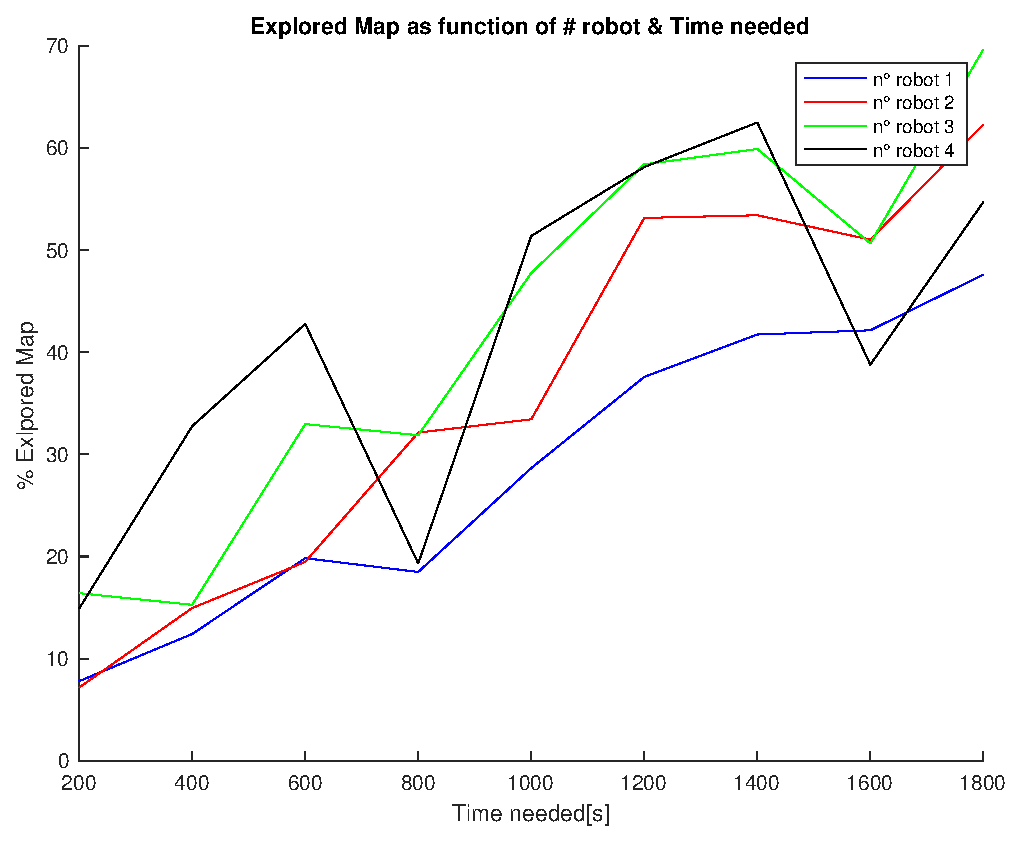
\includegraphics[width=\linewidth]{ExploredMap}
	\caption{Percentuale mappa esplorata per \# robot e tempo di simulazione}
	\label{fig:ExploredMap}
\end{figure}
%
\begin{figure}[htb]
	\centering
	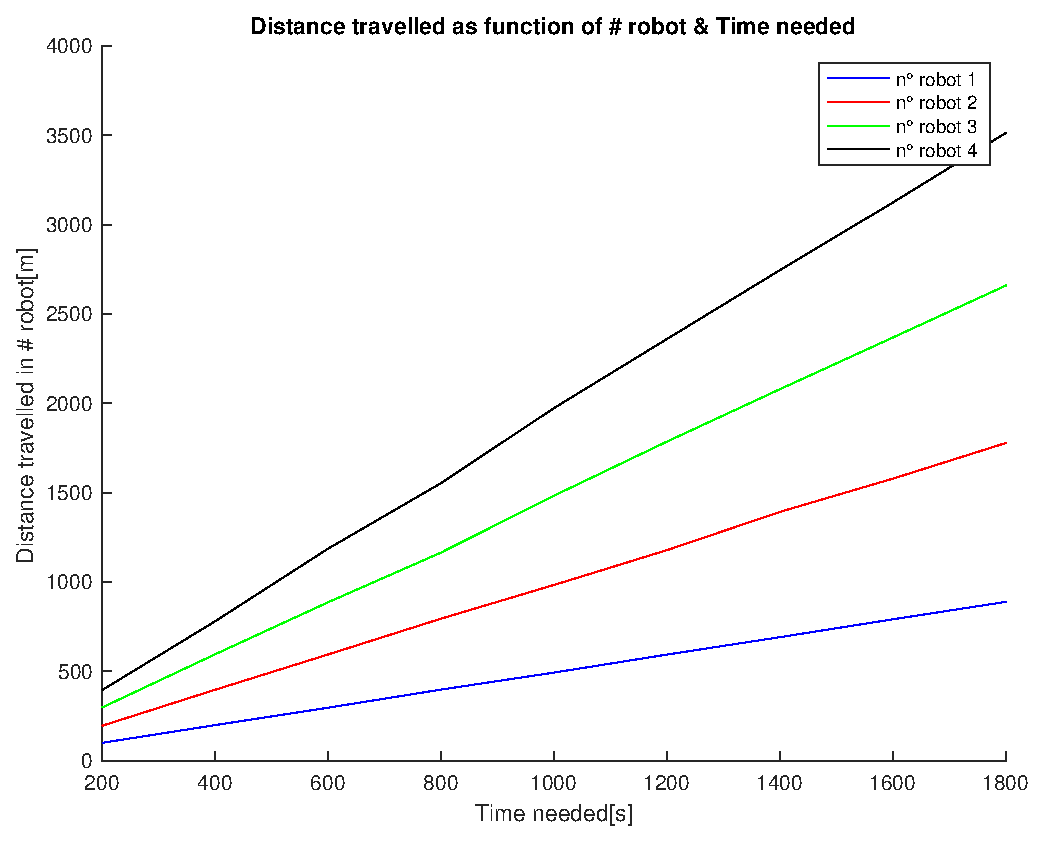
\includegraphics[width=\linewidth]{TotalDistance}
	\caption{Distanza totale percorsa per \# robot e tempo di simulazione}
	\label{fig:TotalDistance}
\end{figure}
\begin{table}[htb]
	\centering
	\caption{Esplorazione su mappa $60 \times 60$}
	\label{tab:optimalresults}
	\begin{tabular}{ccc}
	\toprule
	Test 		& 	Robots		&		Tempo\\
				&	[\#]			&		[\si{\second}]\\
	\midrule
								$\vdots$ & 	$\vdots$ & 	$\vdots$\\
      								33    &		1	 	& 1800\\
		 							34	& 		2 		& 1800\\
	\rowcolor[gray]{.9} 	35	& 		3 		& 1800\\
									36 	& 		4 		& 1800\\
     \bottomrule
\end{tabular}
\end{table}
%
\noindent 
Si evidenzia nella tabella \ref{tab:optimalresults}, il numero ottimo di robot 
e tempo di simulazione che permettono di ottenere le mappe analizzate di seguito.
In figura \ref{fig:IdealMap} viene riportata la mappa fornita dai tre robot in
caso di esplorazione ideale dove il drift non è considerato da parte dei sistemi
robotici.
In figura \ref{fig:RealMap} viene riportata la mappa fornita in caso di presenza
di drift nel sistema e necessità di correzione dello stato dei robot tramite il
particle filter.
\begin{figure}[htb]
	\centering
	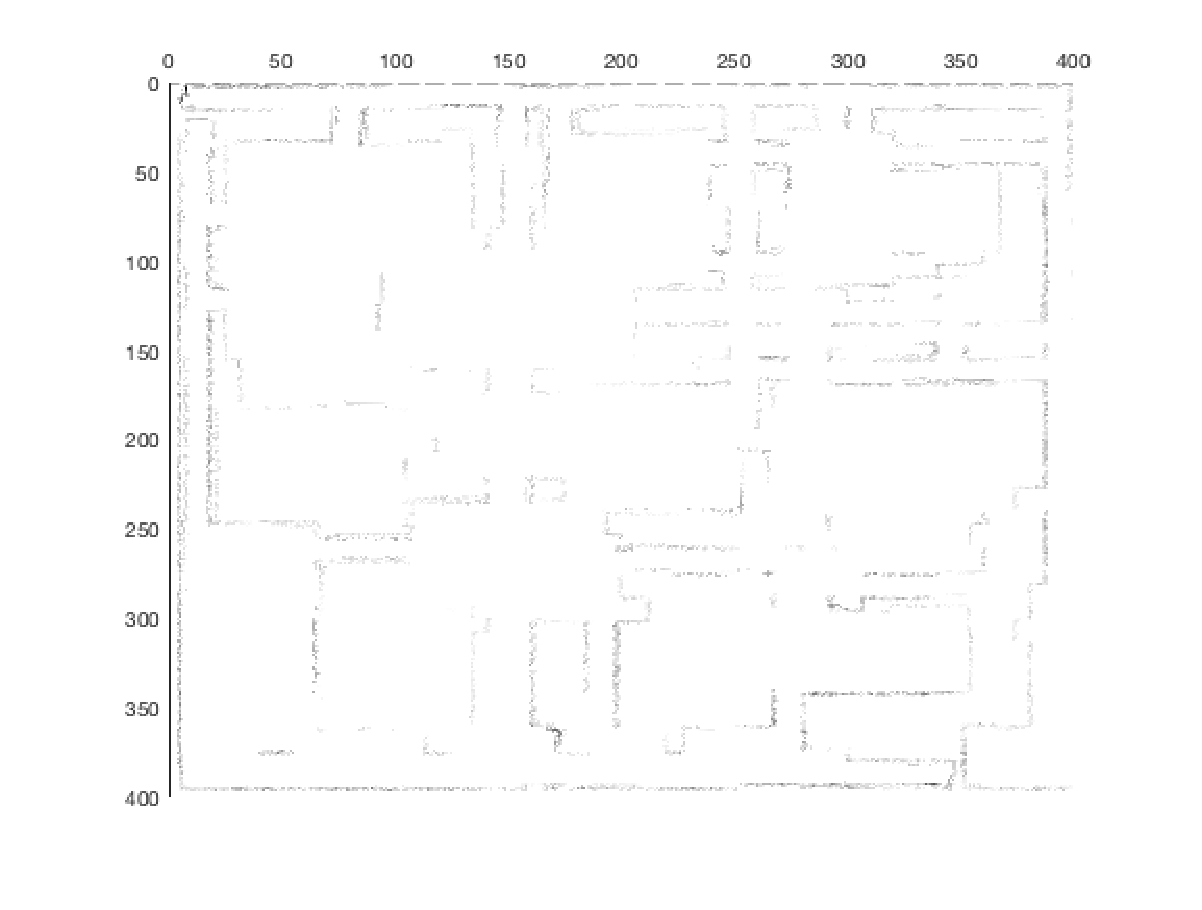
\includegraphics[width=0.95\linewidth]{IdealMap}
	\caption{Mappa fornita dai robot con risoluzione di 0.15 [m] nel caso ideale}
\label{fig:IdealMap}
\end{figure}

\begin{figure}[!htb]
	\centering
	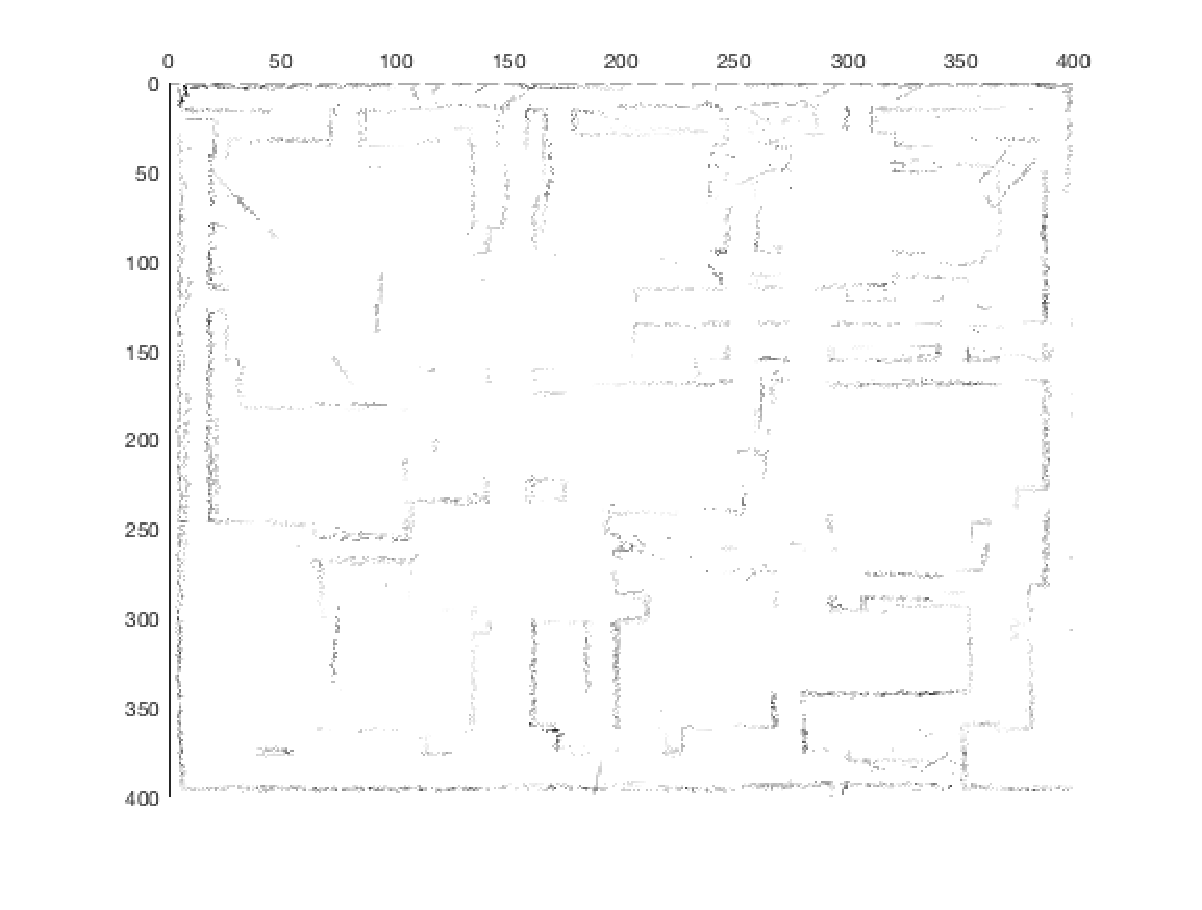
\includegraphics[width=0.95\linewidth]{RealMap}
	\caption{Mappa fornita dai robot con risoluzione di 0.15 [m] nel caso di utilizzo del particle filter }
\label{fig:RealMap}
\end{figure}

Si è deciso di riportare entrambe le mappe per comprendere quali sono gli effettivi 
limiti forniti dal particle filter o della creazione della occupacy grid globale.
Un'altro metodo valutativo per il particle filter risulta essere quello del
calcolo dell'errore quadratico medio fornito dal confronto tra le due traiettorie quelle
stimate(rosse) rispetto a quelle ideali (blu) in figura \ref{fig:maptest}. L'equazione \ref{eq:RMSE} riporta il risultato che considereremo accettabile per la nostra simulazione.

\begin{equation}
RMSE = \sqrt{ \frac{\sum_{k=1}^{k=N}(\hat(x_{k}) - x_{k})^2 }{N}} = 0.442 \si{\metre}
\label{eq:RMSE}
\end{equation}